\documentclass{report}

\usepackage{geometry}
\geometry{a4paper,total={170mm,257mm},left=20mm,top=20mm}
\usepackage[utf8]{inputenc}
\usepackage{amsmath}
\usepackage{amsfonts}
\usepackage{amsthm}
\usepackage{amssymb}
\usepackage{bm}
\usepackage{graphicx}
\usepackage{paralist}
\usepackage[dvipsnames]{xcolor}
\usepackage{caption}
\usepackage{subcaption}
\usepackage{hyperref}
\hypersetup{urlbordercolor=ForestGreen,linkbordercolor=RoyalPurple}
\usepackage{tikz}
\usetikzlibrary{positioning}
\usetikzlibrary{intersections}
\usepackage{algpseudocode}
\usepackage{algorithm}
\usepackage{titling}
\usepackage{pgfplots}
\usepackage{fontawesome5}
 % Use the same header and libraries.
%%% Tento soubor obsahuje definice různých užitečných maker a prostředí %%%
%%% Další makra připisujte sem, ať nepřekáží v ostatních souborech.     %%%

%%% Drobné úpravy stylu

% Tato makra přesvědčují mírně ošklivým trikem LaTeX, aby hlavičky kapitol
% sázel příčetněji a nevynechával nad nimi spoustu místa. Směle ignorujte.
\makeatletter
\def\@makechapterhead#1{
  {\parindent \z@ \raggedright \normalfont
   \Huge\bfseries \thechapter. #1
   \par\nobreak
   \vskip 20\p@
}}
\def\@makeschapterhead#1{
  {\parindent \z@ \raggedright \normalfont
   \Huge\bfseries #1
   \par\nobreak
   \vskip 20\p@
}}
\makeatother

% Toto makro definuje kapitolu, která není očíslovaná, ale je uvedena v obsahu.
\def\chapwithtoc#1{
\chapter*{#1}
\addcontentsline{toc}{chapter}{#1}
}

% Trochu volnější nastavení dělení slov, než je default.
\lefthyphenmin=2
\righthyphenmin=2

% Zapne černé "slimáky" na koncích řádků, které přetekly, abychom si
% jich lépe všimli.
\overfullrule=1mm

%%% Makra pro definice, věty, tvrzení, příklady, ... (vyžaduje baliček amsthm)

\theoremstyle{plain}
\newtheorem{veta}{Věta}
\newtheorem{lemma}[veta]{Lemma}
\newtheorem{tvrz}[veta]{Tvrzení}

\theoremstyle{plain}
\newtheorem{definice}{Definice}
\newtheorem*{pozor}{Pozorování}
\newtheorem*{cvic}{Cvičení}
\newtheorem*{fakt}{Fakt}

\theoremstyle{remark}
\newtheorem*{dusl}{Důsledek}
\newtheorem*{pozn}{Poznámka}
\newtheorem*{prikl}{Příklad}

\theoremstyle{plain}
\newtheorem{thm}{Theorem}
%\newtheorem{lemma}[thm]{Lemma}
\newtheorem{claim}[thm]{Claim}

\theoremstyle{plain}
\newtheorem{defn}{Definition}
\newtheorem*{observ}{Observation}
\newtheorem*{exerc}{Exercise}
\newtheorem*{fact}{Fact}

\theoremstyle{remark}
\newtheorem*{cor}{Corollary}
\newtheorem*{rem}{Remark}
\newtheorem*{example}{Example}


%%% Prostředí pro důkazy

\newenvironment{dukaz}{
  \par\medskip\noindent
  \textit{Důkaz}.
}{
\newline
\rightline{$\qedsymbol$}
}

\newenvironment{myproof}{
	\par\medskip\noindent
	\textit{Proof}.
}{
	\newline
	\rightline{$\qedsymbol$}
}


%%% Prostředí pro sazbu kódu, případně vstupu/výstupu počítačových
%%% programů. (Vyžaduje balíček fancyvrb -- fancy verbatim.)

\DefineVerbatimEnvironment{code}{Verbatim}{fontsize=\small, frame=single}

%%% Prostor reálných, resp. přirozených čísel
\newcommand{\R}{\mathbb{R}}
\newcommand{\N}{\mathbb{N}}
\newcommand{\Z}{\mathbb{Z}}

%%% Užitečné operátory pro statistiku a pravděpodobnost
\DeclareMathOperator{\pr}{\textsf{P}}
\DeclareMathOperator{\E}{\textsf{E}\,}
\DeclareMathOperator{\var}{\textrm{var}}
\DeclareMathOperator{\sd}{\textrm{sd}}

%%% Příkaz pro transpozici vektoru/matice
\newcommand{\T}[1]{#1^\top}

%%% Vychytávky pro matematiku
\newcommand{\goto}{\rightarrow}
\newcommand{\gotop}{\stackrel{P}{\longrightarrow}}
\newcommand{\maon}[1]{o(n^{#1})}
\newcommand{\abs}[1]{\left|{#1}\right|}
\newcommand{\dint}{\int_0^\tau\!\!\int_0^\tau}
\newcommand{\isqr}[1]{\frac{1}{\sqrt{#1}}}

%%% Vychytávky pro tabulky
\newcommand{\pulrad}[1]{\raisebox{1.5ex}[0pt]{#1}}
\newcommand{\mc}[1]{\multicolumn{1}{c}{#1}}


% set up \maketitle to accept a new item
\predate{\begin{center}\placetitlepicture\large}
	\postdate{\par\end{center}}

% commands for including the picture
\newcommand{\titlepicture}[2][]{%
	\renewcommand\placetitlepicture{%
		\includegraphics[#1]{#2}\par\medskip
	}%
}
\newcommand{\placetitlepicture}{} % initialization

 % Use global macros.

\usepackage{babel}

\title{Geometrická reprezentace grafů}
\author{Tomáš Turek}
\titlepicture[width=6in]{res/filament}
\date{\today}

\begin{document}
	\maketitle
	
	\INFO{Many parts of text are taken from the handouts made by Jan Kratochvíl. I also add some of my notes from the lectures and some pictures.}
	
	\tableofcontents
	\part{Geometrická reprezentace grafů I}
	\chapter{Introduction}

Firstly we remind some basics from flows and cuts. 

\section{Network flow}

\textbf{Flow} is defined on a \textbf{network}. Network is on a oriented graph $G = (V,E)$ and it has two special vertices $s,t \in V$ called source and target. Also we have a capacity, which is a mapping $c : E \to \R_{0}^{+}$. Flow then is a mapping $f : E \to \R_{0}^{+}$ which has two properties.

\begin{enumerate}
	\item $\forall e \in E: f(e) \leq c(e)$
	\item Kirchoff's law: $\forall v \neq s, t \in V: \sum_{uv \in E} f(uv) - \sum_{vu \in E} f(vu) = 0$
\end{enumerate}

\section{Min $s,t$-cut}

Now we also remind ourselves another term which is an $s,t$-cut. Which is a $M \subset E$ such that no $s,t$-path exists in $G' = (V, E \setminus M)$.

These basic terms can be generalized to a \textbf{multi-commodity flow} problem and \textbf{multi-cut} problem.
	\chapter{Interval, permutation and function graphs}

\section{Interval graphs}

\begin{defn}
	A graph is an \textbf{interval graph} if it is isomorphic to the intersection graph of a collection of intervals on a line.
\end{defn}

\begin{observ}
	Every interval graph has an interval representation in which all of the intervals are closed.
\end{observ}

\begin{defn}[Clique-path decomposition]
	A \textbf{clique-path decomposition} of a graph is a clique-tree decomposition in which the underlying tree is a path.
\end{defn}

\begin{thm}
	For any graph $G$, the following statements are equivalent:
	
	\begin{enumerate}
		\item $G$ is an interval graph,
		\item $G$ has a clique-path decomposition, and
		\item $G$ is an intersection graph of subpaths of a path.
	\end{enumerate}
\end{thm}

\begin{proof}
	"$1. \Leftrightarrow 3.$" is obvious.
	
	"$1. \Rightarrow 2.$" Assume $I_u , u \in V(G$ is an interval representation of $G$. Use the fact that intervals on a line have the Helly property, i.e., if any two of a collection of intervals have a nonempty intersection, then all of them have a nonempty intersection. In other words, if $Q_i \in \mathcal{Q}$ is a maximal clique of $G$, then there exists a point $P_i$ which belongs to $\bigcap_{u \in Q_i} I_u$ . Moreover, for every $v \notin Q_i , P_i \notin I_v$, since $Q_i$ is a maximal clique. (E.g., the rightmost of the left endpoints of the intervals $I_u , u \in Q_i$ is a good candidate for $P_i$.) Order the cliques of $Q$ as $Q_1, Q_2, \dots, Q_k$ so that $P_1 < P_2 < \dots < P_k$. Then the path
	$Q_1 Q_2 \dots Q_k$ is a clique-path decomposition of $G$.
	
	"$2. \Rightarrow 3.$" Given a clique-path decomposition $P = (\mathcal{Q}, F)$, define $P_u = P [\{Q : u \in Q \in \mathcal{Q}\}]$ for $u \in V(G)$. Clearly $V(P_u) \cap V(P_v) \neq \emptyset$ iff $u$ and $v$ belong to the same maximal clique of $G$, which happens if and only $u$ and $v$ are adjacent in $G$.
\end{proof}

\section{Comparability graphs}

\begin{defn}
	A graph $G$ is a \textbf{comparability graph} if there exists a partial order $P = (V(G), \leq)$ on the vertex set of $G$ (i.e., an \textbf{antireflexive}, \textbf{antisymmetric} and \textbf{transitive binary relation}) such that for any two vertices $u, v \in V(G)$, $uv \in E(G)$ if and only if $u \leq v$ or $v \leq u$ (i.e., if $u$ and $v$ are comparable in $P$). The class of comparability graphs will be denoted by CO.
\end{defn}

\begin{observ}
	A graph is a comparability graph if and only if its edges can be transitively oriented.
\end{observ}

\begin{notation}
	If $\mathcal{A}$ is a graph class, the symbol $\text{co}-\mathcal{A}$ is used to denote the class containing the complements of the graphs in $\mathcal{A}$.
\end{notation}

\begin{observ}
	If $A \subseteq B$, then $\text{co}-A \subseteq \text{co}-B$.
\end{observ}

\begin{thm}
	All equivalencies hold:
	
	\begin{enumerate}
		\item $\text{FUN} = \text{co}-\text{CO}$
		\item $\text{PER} = \text{CO} \cap \text{co}-\text{CO}$
		\item $\text{INT} = \text{CHOR} \cap \text{co}-\text{CO}$
	\end{enumerate}
\end{thm}

\begin{proof}
	\begin{enumerate}
		\item ”FUN $\subseteq$ co-CO”: Given a collection of curves joining two vertical parallel lines (and lying in the stripe between them), for any two non-crossing curves, it is uniquely determined which one lies above the other one (this follows from the Jordan curve theorem), and this gives a transitive orientation of the complement of the intersection graph of this collection.
		
		”co-CO $\subseteq$ FUN”: Let $G = (V, E)$ be a graph and let $P = (V, \leq)$ be a partial order which corresponds to a transitive orientation of the complement of $G$. If $d$ is the dimension of $P$, $P$ is the intersection of $d$ linear orders $L_1, L_2 , \dots, L_d$ of $V$. In the plane, draw d distinct parallel (vertical) lines $l_1, l_2, \dots, l_d$, and on each $l_i$ , mark distinct points $P_{iu}, u \in V$ bottom up in the order $L_i$. Consider piece-wise linear curves $c(u) = P_{1u} P_{2u} \dots P_{du}$, for $u \in V$. If $uv \in E$, $u$ and $v$ are incomparable in $P$,	and hence there are indices $i$ and $j$ such that $u <_{L_i} v$ and $v <_{L_j} u$, in other words $P_{iu}$ is below $P_{iv}$, while $P_{ju}$ is above $P_{jv}$. Hence the curves $c(u)$ and $c(v)$ cross somewhere between $l_i$ and $l_j$. If, on the other hand, $uv \notin E$, $uv$ is an edge of the complement of $G$ and hence $u$ and $v$ are comparable in $P$, say, $u \leq v$. But then $u <_{L_i} v$ for every $i = 1, 2, \dots, d$, and for each $i = 1, 2, \dots, d - 1$, the curve $c(u)$	lies below the curve $c(v)$ in the stripe between $l_i$ and $l_{i+1}$. Thus $c(u)$ and $c(v)$ are disjoint.
		
		\item Note first that co-PER $\subseteq$ PER. Indeed, given a permutation representation of a graph, swap	the order of the endpoints on one of the bounding lines to obtain a representation of the complement of the given graph. Then PER $=$ co-(co-PER) $\subseteq$ co-PER, and hence PER $=$ co-PER.
		
		”PER $\subseteq$ CO $\cap$ co-CO”: Obviously PER $\subseteq$ FUN $=$ co-CO. Then the above small observation implies PER $=$ co-PER $\subseteq$ co-(co-CO) $=$ CO as well.

		”CO $\cap$ co-CO $\subseteq$ PER”: Suppose both $G$ and its complement can be transitively oriented, say $\overrightarrow{E_1}$ be a transitive orientation of $G$ and $\overrightarrow{E_2}$ a transitive orientation of the complement $-G$ of $G$. Then $\overrightarrow{E_1} \cup \overrightarrow{E_2}$ is a transitive orientation of the complete graph $K_{V(G)}$ on the vertex set of $G$, i.e., a linear ordering of the vertices of $G$. And so is $\overrightarrow{E_1}^{-1} \cup \overrightarrow{E_2}$. Place the vertices of $G$ on two parallel lines, on one of them in the linear order given by $\overrightarrow{E_1} \cup \overrightarrow{E_2}$, on the other one in the order given by $\overrightarrow{E_1}^{-1} \cup \overrightarrow{E_2}$, and connect the two occurrences of a vertex $u$ by a straight-line segment called $s(u)$, for every vertex $u \in V(G)$. If $uv \in E(G)$, then the pair $u, v$ is ordered differently on the two lines (by $\overrightarrow{E_1}$ on one of them and by $\overrightarrow{E_1}^{-1}$ on the other one) and the segments $s(u), s(v)$ cross each other somewhere between	the two lines. If $uv \notin E(G)$, the pair $u, v$ is ordered the same way (by $\overrightarrow{E_2}$) on both of the lines, and thus the segments $s(u)$ and $s(v)$ are disjoint. So $\{s(u)\}_{u \in V(G)}$ is a permutation representation of $G$.
		
		\item ”INT $\subseteq$ CHOR $'cap$ co-CO”: Let $\{I(u)\}_{u \in V(G)}$ be an interval representation of a graph $G$. Define a transitive orientation $\overrightarrow{E_2}$ of the non-edges of $G$ by setting $uv \in \overrightarrow{E_2}$ if $\max I(u) < \min I(v)$. Thus $G \in$ co-CO. The fact that $G \in$ CHOR follows from the fact that
		
		$$
		\text{INT} = \mathcal{IG}(\{\text{connected subgraphs of paths}\}) \subseteq
		$$
		
		$$
		\subseteq \mathcal{IG}(\{\text{connected subgraphs of trees}\}) = \text{CHOR}.
		$$
		
		”CHOR $\cap$ co-CO $\subseteq$ INT”: Let $G$ be a chordal graph which allows a transitive orientation $\overrightarrow{E_2}$ of its non-edges. Define a binary relation $<$ on the set $\mathcal{Q}$ of maximal cliques of $G$ by setting
		
		$$
		Q < Q' \Leftrightarrow \exists u \in Q \exists v \in Q' : uv \in \overrightarrow{E_2}.
		$$
		
		\begin{claim}
			The relation $<$ is a partial order on $\mathcal{Q}$.
		\end{claim}
		
		\begin{proof}[Proof of claim]
			We will show all properties of partial order.
			\begin{itemize}
				\item Antireflexivity: Each $Q \in \mathcal{Q}$ is a clique, so there are no two vertices $u, v \in Q$ that would form a	non-edge of $G$. Hence $Q \not< Q$.
				
				\item Antisymmetry: Suppose for the contrary that there are $u \in Q, v \in Q'$ s.t. $uv \in \overrightarrow{E_2}$, and another pair $x \in Q, y \in Q'$ s.t. $yx \in \overrightarrow{E_2}$. First observe that $u \neq x$ and $v \neq y$ (if $u = x$, the transitivity of $\overrightarrow{E_2}$ would imply $yv \in \overrightarrow{E_2}$, which is impossible; if $v = y$, the transitivity of $\overrightarrow{E_2}$ would imply $ux \in \overrightarrow{E_2}$, which is again impossible). Next observe that both $uy$ and $xv$ must be edges of $G$ (if $uy \notin E(G)$, then either $uy \in \overrightarrow{E_2}$, or $yu \in \overrightarrow{E_2}$, yielding $ux \in \overrightarrow{E_2}$ in the former case and $yv \in \overrightarrow{E_2}$ in the letter one, both contradicting the fact that $Q$ and $Q'$ are cliques of $G$; the case of $xv \notin E(G)$ is analogous). Lastly, we conclude that $G[\{u, v, x, y\}] \simeq C_4$ , contradicting the assumption that $G$ is chordal.
				
				\item Transitivity: Suppose $Q < Q' < Q''$ and let $u \in Q, v, x \in Q'$ and $y \in Q''$ be vertices such that $uv, xy \in \overrightarrow{E_2}$. If $v = x$, the transitivity of $\overrightarrow{E_2}$ implies $uy \in \overrightarrow{E_2}$, hence $Q < Q''$. If $v \neq x$, one of $ux$, $vy$
				must be a non-edge (otherwise $G[\{u, v, x, y\}]$ would be an induced cycle of length 4, contradicting the assumption that $G$ is chordal). If $ux \notin E(G)$, $ux \in \overrightarrow{E_2}$ and the transitivity of $\overrightarrow{E_2}$ implies $uy \in \overrightarrow{E_2}$. If $vy \notin E(G)$, $vy \in \overrightarrow{E_2}$ and the transitivity of $\overrightarrow{E_2}$ implies $uy \in \overrightarrow{E_2}$. In either case, $Q < Q''$.
			\end{itemize}
		\end{proof}
		
		\begin{claim}
			The relation $<$ is a linear ordering of $\mathcal{Q}$.
		\end{claim}
		
		\begin{proof}[Proof of claim]
			Let $Q \neq Q'$ be two different maximal cliques of $G$. Their maximality implies that none of them is a subset of the other one. Hence there is a vertex $u \in Q$ which does not belong to $Q'$ . If $u$ were adjacent to all vertices of $Q'$, $Q' \cup \{u\}$ would be a clique of $G$, contradicting the maximality of $Q'$ . Hence there is a $v \in Q'$ such that $uv \notin E(G)$. Then either $uv \in \overrightarrow{E_2}$ or $vu \overrightarrow{E_2}$, thus $Q < Q'$ or $Q' < Q$.
		\end{proof}
		
		\begin{claim}
			Let $\mathcal{Q} = \{Q_1 < Q_2 < \dots < Q_k\}$ be the maximal cliques of $G$ ordered by $<$. Then $P_G = (\mathcal{Q}, \{Q_i Q_{i+1}: i = 1, 2, \dots, k - 1\})$ is a clique-path decomposition of $G$, and hence $G \in$ INT.
		\end{claim}
		
		\begin{proof}[Proof of claim]
			Indeed $P_G$ is a path whose nodes are the maximal cliques of $G$. It remains to show that vertices of $G$ appear in these cliques consecutively. Suppose $Q < Q' < Q''$ and $u \in Q \cap Q''$. If there were a vertex $v \in Q'$ nonadjacent to $u$, we would have $uv \in \overrightarrow{E_2}$ because of $Q < Q'$ and $vu \in \overrightarrow{E_2}$ because of $Q' < Q''$, contradicting the antisymmetry of $\overrightarrow{E_2}$. Hence $u$ is adjacent to all vertices of $Q'$ , and thus
			$u \in Q'$ follows from the maximality of $Q'$.
		\end{proof}
	\end{enumerate}
\end{proof}
	\chapter{Interval filament graphs}

\begin{defn}
	Given a half-plane $\pi$ with a border-line $l$, an \textbf{interval filament} in $\pi$ is a simple curve with
	endpoints on $l$, its interior lying in $\pi$ and within the stripe determined by lines perpendicular to $l$ and
	passing through the endpoints of the curve. The class of \textbf{interval filament graphs} is $\text{IFA} = \mathcal{IG}\{\text{interval filaments in a half-plane}\}$.
\end{defn}

\begin{figure}[!ht]\centering
	\begin{tikzpicture}
		\draw[color = gray] (2,0) -- (10,0);
		\node at (3,.3) {$l$};
		\draw[color=black, thick] (5,.01) edge (10,.01);
		\draw[dotted] (5,0) edge (5, 5);
		\draw[dotted] (10,0) edge (10,5);
		
		\draw[color=Red, thick] (5, .01) .. controls (10,5) and (4,3) .. (7, 4);
		\draw[color=Red, thick] (7, 4) .. controls (11,1) and (1,1) .. (10, .01);
		
		\fill[color=Red] (7,4) circle[radius=.35pt];
	\end{tikzpicture}
	\caption{An illustration to the definition. The name “interval-filament” comes from the fact that the curve “lives above” the interval that is determined by the endpoints of the filament on the boundary line $l$.}
\end{figure}

\begin{comm}
	If the base intervals of two interval-filaments overlap (i.e., they are not disjoint, but none of them is a subinterval of the other one), the filaments necessarily cross each other and the corresponding vertices in the intersection graph are adjacent (cf. the blue and red filaments in Fig. \ref{filaments}). On the other hand, if one of the base intervals is included in the other one, their filaments may or may not be disjoint (cf. the blue and yellow filaments for the disjoint case, and the red and green filaments for the non-disjoint one, both in Fig. \ref{filaments}).
\end{comm}

\begin{figure}[!ht]\centering
	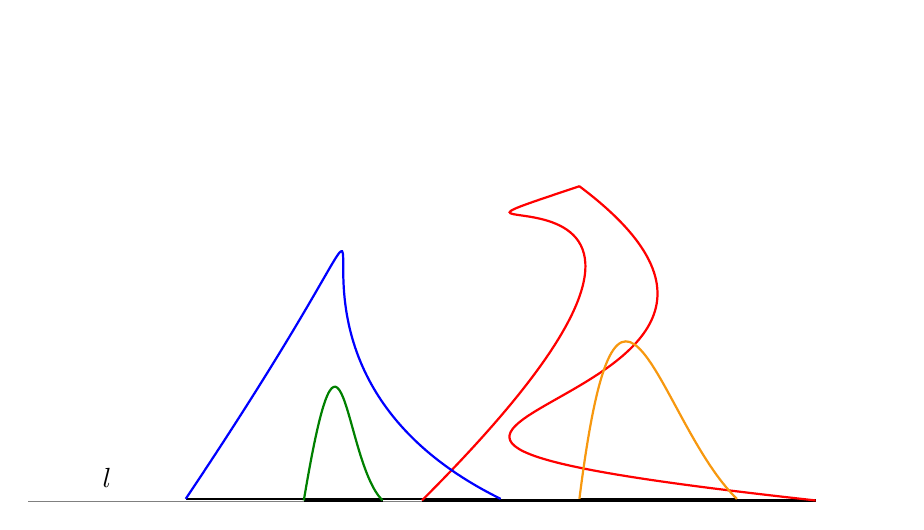
\begin{tikzpicture}
		\draw[color = gray] (0,0) -- (10,0);
		\node at (1,.3) {$l$};
		
		\draw[color=black, thick] (5,.01) edge (10,.01);
		\draw[color=black, thick] (7,.03) edge (9,.03);
		\draw[color=black, thick] (2,.03) edge (6,.03);
		\draw[color=black, thick] (3.5,.01) edge (4.5,.01);
		
		\draw[color=Red, thick] (5, .01) .. controls (10,5) and (4,3) .. (7, 4);
		\draw[color=Red, thick] (7, 4) .. controls (11,1) and (1,1) .. (10, .01);
		\fill[color=Red] (7,4) circle[radius=.35pt];
		
		\draw[color=Green, thick] (3.5, .01) .. controls (4,3) and (4,.5) .. (4.5, .01);
		\draw[color=Blue, thick] (2, .03) .. controls (6,6) and (2,2) .. (6, .03);
		\draw[color=YellowOrange, thick] (7, .03) .. controls (7.5,4) and (8,1) .. (9, .03);
	\end{tikzpicture}
	\caption{An illustration to the possible relative positions of interval-filaments.}
	\label{filaments}
\end{figure}
	\chapter{Cliques and independent sets}

We will show the computational complexity of the following optimization problems:

\begin{itemize}[]
	\item \textbf{Clique}
	\item \textit{Input:} A graph $G$.
	\item \textit{Output:} $\omega(G)$.
\end{itemize}

and

\begin{itemize} []
	\item \textbf{Independent Set}
	\item \textit{Input:} A graph $G$.
	\item \textit{Output:} $\alpha(G)$.
\end{itemize}

and their weighted variants

\begin{itemize}[]
	\item \textbf{Weighted Clique}
	\item \textit{Input:} A graph $G$ and a non-negative weight function $w : V(G) \to R_0^+$.
	\item \textit{Output:} A clique $C \subseteq V(G)$ which maximizes $w(C) = \sum_{u \in C} w(u)$.
\end{itemize}

and

\begin{itemize}[]
	\item \textbf{Weighted Independent Set}
	\item \textit{Input:} A graph $G$ and a non-negative weight function $w : V(G) \to R_0^+$.
	\item \textit{Output:} An independent set $A \subseteq V(G)$ which maximizes $w(A) = \sum_{u \in A} w(u)$.
\end{itemize}

Our goal is to show that for many of the intersection-defined graph classes that we have seen so far, these problems can be solved in polynomial time. For the sake of brevity, we denote by $\omega_w(G)$ the maximum possible weight $w(C)$ over all cliques $C$ in $G$, and by $\alpha_w(G)$ the maximum possible weight $w(A)$ over all independent sets $A$ in $G$.

\section{Interval graphs}

\begin{thm}
	\textbf{Weighted Clique} can be solved in polynomial time for interval graphs.
\end{thm}

\begin{proof}
	Interval graphs have only linearly many maximal cliques. We look at all of them and compare
	their weights.
\end{proof}

\begin{thm}
	\textbf{Weighted Independent Set} can be solved in polynomial time for interval graphs.
\end{thm}

\begin{proof}
	Suppose we are given an interval intersection representation $\mathcal{R} = \{I_u = [l_u , r_u] : u \in V\}$ of	a graph $G = (V, E)$, equipped with a weight function $w$. We may assume that all endpoints of the intervals are different. Number the endpoints $P_1 , P_2 , \dots , P_{2n}$ so that $P_i < P_{i+1}$ for $i = 1, 2, \dots , 2n - 1$.	Use dynamic programming to compute $w_i$ which is defined as the maximum possible weight of an	independent set $A$ in $G$ such that $r_u < P_i$ for all $u \in A$. This can be computed as follows:
	
	\begin{algorithm}[!ht]
		\begin{algorithmic}[1]
			\State $w_i := 0$
			\For{$i := 1$ to $2n$}
				\If{$P_i$ is the left endpoint of an interval}
					\State $w_{i+1} := w_i$
				\Else
					\State let $u \in V$ be such that $r_u = P_i$ and let $j$ be such that $P_j = l_u$;
					\State set $w_{i+1} = \max \{w_j + w(u), w_i\}$
				\EndIf
			\EndFor
			\State \Return $w_{2n+1}$
		\end{algorithmic}
	\end{algorithm}
\end{proof}

\begin{cor}
	\textbf{Weighted Clique} and \textbf{Weighted Independent Set} can both be solved in polynomial	time on co-INT graphs.
\end{cor}

\section{Comparability graphs}

\begin{thm}
	\textbf{Weighted Clique} can be solved in polynomial time for comparability graphs.
\end{thm}

\begin{proof}
	Given a transitive orientation $\overrightarrow{E}$ of $G = (V, E)$, order the vertices linearly $V = \{v_1 , v_2 , \dots, v_n\}$ in a topological sorting according to $\overrightarrow{E}$ (i.e., $v_i v_j \in \overrightarrow{E}$ implies $i < j$). For each $i$, set $W_i = \{j : v_j v_i \in E\}$ and let $w_i$ be the maximum weight $w(C)$ over all cliques $C \subseteq W_i \cup \{v_i\}$. Note that if $w(v_i) > 0$, each clique attaining the maximum weight contains $v_i$, and we may consider without loss	of generality only the cliques that contain $v_i$ even if $w(v_i) = 0$. The values $w_i , i = 1, 2, \dots , n$ can be computed recursively as follows
	
	\begin{algorithm}[!ht]
		\begin{algorithmic}[1]
			\For{$i := 1$ to $n$}
				\State $w_i := \max_{j \in W_i} w_j + w(v_i)$
			\EndFor
		\end{algorithmic}
	\end{algorithm}
	
	and clearly $\omega_w(G) = max_{i=1}^n w_i$.
\end{proof}

\begin{thm}
	\textbf{Weighted Independent Set} can be solved in polynomial time for \\ comparability graphs.
\end{thm}

\begin{proof}
	Given a transitive orientation $\overrightarrow{E}$ of $G = (V, E)$, consider the partial order $P = (V, \overrightarrow{E})$ determined by this orientation. The weighted version of Dilworth theorem yields that $\alpha_w(P)$ is equal to the minimum cost of a flow in the network $N = (V \cup \{s, t\}, E \cup \{su, ut : u \in V\})$ with vertex demands $f(u) \geq w(u)$, and this can be computed in polynomial time by network flow algorithms.
\end{proof}

\begin{cor}
	\textbf{Weighted Clique} and \textbf{Weighted Independent Set} can both be solved in polynomial time on function (= co-comparability) graphs.
\end{cor}

\section{Interval-filament graphs}

In this section we show the strongest results. Note, however, that we need the input graph to be given with an interval-filament representation (or, equivalently, with a partition of its edge set satisfying the mixing property).

\begin{thm}
	\textbf{Weighted Clique} can be solved in polynomial time for interval-filament graphs, if an interval-filament representation is provided on the input.
\end{thm}

\begin{proof}
	
\end{proof}
\end{document}

